\documentclass[12pt]{report}

\usepackage{graphicx}
\usepackage[spanish]{babel} % Para separar correctamente las palabras
\usepackage[utf8]{inputenc} % Este paquete permite poner acentos y eñes usando codificación utf-8
\usepackage{setspace}
\onehalfspace %para espacio y medio

\usepackage{fancyhdr} %encabezado y pie de pag
\usepackage{framed} %recuadros de texto
\usepackage{multicol} %colocar texto en columnas

% Title Page
\title{Análisis de Identificadores para Abstraer conceptos del Dominio del Problema}
\author{Javier Azcurra\\\\Trabajo Final de Licenciatura en Cs. de la Computación\\\\\\Facultad de Ciencias Físico Matemáticas y Naturales\\Universidad Nacional de San Luis}

%\begin{figure}[h] %[h] para here [b] para bottom [t] para top
%\centering
%
\includegraphics[scale= 0.18]{./unsl_logo.JPG}
%\caption{Gráfico de Comprensión de Programas}
%\end{figure} \label{captura1}

%Encabezado
\lhead[]{\leftmark}
\chead[]{}
\rhead[]{\thepage}
\renewcommand{\headrulewidth}{0pt}

%Pie de pag
\lfoot[]{}
\cfoot[]{}
\rfoot[]{}
\renewcommand{\footrulewidth}{0pt}

%Setea configuracion enc y pie de pag
\pagestyle{fancy}


\begin{document}
\maketitle

%\renewcommand{\abstractname}{Agradecimientos}
%\begin{abstract}
%\begin{multicols}{2}
%\begin{flushleft}
%\end{flushleft}
%\columnbreak
%\begin{flushright}
%\textbf{{\large \textit{“Hay en el mundo un lenguaje que todos comprenden: es el lenguaje del entusiasmo, de las cosas hechas con amor y con voluntad, en busca de aquello que se desea o en lo que se cree.”\linebreak\linebreak Paulo Cohelo}}}
%\end{flushright}
%\end{multicols}
%\end{abstract}

\begin{abstract}
Las demandas actuales en el desarrollo del software implican una evolución y mantenimiento constante del mismo con el menor costo de tiempo y de recursos. Pensar en estrategias que faciliten las tediosas tareas que diariamente conllevan al crecimiento de los sistemas nos da incapie a iniciarnos en la investigación de herramientas automatizadas que posibiliten el reemplazo del esfuerzo manual que realizan los ingenieros de software a la hora de interpretar un programa.

Estudios indican que los identificadores abundan en los códigos de programas y poseen información relevante detrás de sus abreviaturas por lo tanto no debe ser pasados por alto su análisis cuando se están elaborando herramientas automatizadas de interpretación de códigos.
El correspondiente trabajo habla de técnicas basadas en el análisis de identificadores en códigos escritos en lenguaje JAVA\texttrademark .
Se utilizan técnicas de compilación para capturar identificadores.
Luego las técnicas de análisis de identificadores constan de dos etapas la primera consiste en la división de las distintas abreviaturas que componen un identificador y la segunda etapa se encarga de la expansión “semántica” de cada abreviatura obtenida en la etapa previa, es decir, expandir las abreviaciones en palabras completas. Para lograr esta expansión se emplean distintas fuentes compuestas de información informal: comentarios, literales, documentación o bien con fuentes externas al sistema basándose en diccionarios. Cada una de las estrategias de análisis de identificadores utilizan distintas políticas es por ello que algunas se implementaron en la herramienta \textit{Identifier Analyzer} (IDA) con el objetivo de poder comparar el desempeño de cada estrategia en base a distintos casos de estudio y así arribar a conclusiones.

\end{abstract}

\tableofcontents %Genera el indice

%CAPITULO1=============================================================

\chapter{Introducción}
\section{Problema}


La ingeniería de software contiene tres temáticas muy importantes en desarrollo de los sistemas: el \textit{mantenimiento del software}, la \textit{evolución del software} y la \textit{migración del software}. Para que puedan llevar a cabo sus iniciativas las tres necesitan interpretar previamente el sistema que se esta desarrollando.

La etapa de mantenimiento es importante en el desarrollo de un software ya que este esta sujeto a cambio y a una permanente evolución\cite{PFT02}.
Es común también que por la constate actualización de los sistemas operativos, los motores de base de datos y demás sistemas externos que interactúan con el software desarrollado entren en conflicto, por eso en la fase de mantenimiento también se debe ir actualizando los distintos componentes del producto para una mejor compatibilidad.\cite{RSPMGH02}. Por lo antedicho entre otras diversas razones indican que el mantenimiento del software consume mucho esfuerzo y dinero. Es necesario pensar en estrategias de automatización que puedan ser aplicadas en fases del mantenimiento del software que ayuden a reducir estos costos, para lograrlo se requiere una comprensión del objeto que se va a modificar antes de realizar algún cambio que sea de utilidad.


Los sistemas complejos evolucionan con el tiempo, los nuevos usuarios y requisitos durante el desarrollo del mismo causan que el producto final posiblemente no sea el que se planteó en un comienzo. 
Generalmente los ingenieros del software utilizan modelos de procesos conocidos que se diseñan de antemano para adaptarse a un producto que evoluciona con el tiempo, estos modelos se conocen con el nombre de modelos evolutivos o modelos iterativos, este ultimo hace referencia a que el ingeniero del software obtenga una versión entregable del producto cada vez más completa en cada iteración, esto se considera importante ya que las fechas ajustadas y el mercado competitivo obligan a entregar una versión funcional limitada lo más rápido posible y no esperar a tener una única versión completa al final del proceso de desarrollo\cite{RSPMGH02}.
La evolución del software básicamente se atribuye al crecimiento de los sistemas, es decir, tomar una versión operativa y generar una nueva versión ampliada, para lograrlo se necesita previamente una correcta y eficiente interpretación del sistema.


La migración del software es una tarea fundamental y compleja dentro del mantenimiento del software. El objetivo es convertir un viejo sistema dentro de una nueva tecnología sin cambiar la funcionalidad del mismo, lograr esto es costoso \cite{WHAFVR11}. Las migraciones de sistemas mas comunes que se conocen son iniciadas por cambios en el hardware, sistemas operativos, arquitectura, interfaces web, base de datos, entre otras mas \cite{MMFAF07}. Es importante lograr una buena comprensión del sistema antiguo, una forma de alcanzarlo es elevar el código antiguo a un nivel más alto de abstracción tomando las principales características.

%WICC:
De todos los problemas a los que se enfrentan los desarrolladores de software el primordial es el de mantener los sistemas en buen funcionamiento \cite{VMAVA95}. 
Esta tarea es imposible de llevar a cabo de forma manual debido a que consume muchos costos y esfuerzo humano. 
Por esta razón, existe una área de la Ingeniería de Software que se  
dedica al desarrollo de técnicas de inspección y comprensión de software. 
Esta área tiene como principal objetivo que el desarrollador logre un entendimiento 
acabado del software de estudio de forma tal de poder modificarlo disminuyendo en lo posible la gran mayoría de costos \cite{BRM10}. 
El área mencionada se conoce en la jerga de la Ingeniería de Software como: \textit{Comprensión de Programas (CP)}.

La CP es una rama de la Ingeniería de Software cuyo objetivo 
principal es desarrollar métodos, técnicas y herramientas que faciliten al programador 
el entendimiento de las funcionalidades de los sistemas de software.
Una forma de alcanzar este objetivo consiste en relacionar el Domino del Problema, 
es decir la salida del sistema, con el dominio del programa, o sea 
con las partes del programa utilizadas para generar la salida del sistema.
\textbf{La construcción de esta relación representa el principal desafío en el contexto de la CP.}

%==============================================================================


\section{Solución}

\textbf{Una solución que se aproxime al desafío previamente mencionado consiste en construir una representación para el dominio del problema y otra para el dominio del programa luego unir ambas representaciones utilizando una estrategia de vinculación} 
El camino que facilita la vinculación de las dos representaciones consiste en el uso/creación de Herramientas de Comprensión. 
Una Herramienta de Compresión presenta diferentes perspectivas del software que posibilitan que el ingeniero pueda percibir el funcionamiento del sistema. 
Para construir herramientas de comprensión, se deben tener en cuenta cuatro pilares importantes: \textit{Modelos Cognitivos}
\textit{Extracción de la Información},
\textit{Interconexión de Dominios} y la
\textit{Visualización de Software} \cite{STOREY99,BROOK82}.


Los \textit{Modelos Cognitivos} se refiere a las estrategias de estudio y las estructuras de información usadas por los programadores para comprender los programas. Están formados por distintos componentes: Conocimiento, un modelo mental y un proceso de asimilación.
Existen dos tipos de conocimientos uno es el interno que constituye los conocimientos que el programador tiene incorporado y el otro es el Externo en donde el sistema a estudiar provee al desarrollador nuevos conceptos.
El modelo mental es la representación mental que el programador tiene sobre el sistema. Algunos modelos conocidos por los arquitectos del software como el \textit{Unified Modeling Language} UML, \textit{Entity Relationship} ER entre otros pueden verse como representaciones de modelos mentales.
Por último, el proceso de asimilación engloba la estrategia que utiliza el programador para entender los programas. Ellas son Botton-up, Top-Down e Hibrida.
Varios autores concluyen que estos conceptos conforman la base para encontrar la relación entre el dominio del problema y el dominio del programa\cite{TIE89,MPOB03}.


La \textit{Visualización del Software} es una característica importante en la comprensión de programas, básicamente provee una o varias representaciones visuales (o vistas) de algún sistema particular \cite{BRM10}.
Dichas vistas, cuando están bien elaboradas, permiten analizar y percibir la información extraída desde un programa con mayor facilidad.
Para lograr lo antedicho se utilizan librerías gráficas conocidas, algunas de ellas son Jung, Prefuse, Graphviz y Cairo.
Cabe destacar que el diseñador de la visualización debe hacer un análisis profundo para seleccionar la librería mas adecuada.
La visualización de software orientada a la comprensión de programa tiene como principal desafío generar vistas que ayuden a relacionar el Dominio del Problema con el Dominio del Programa.

La \textit{Interconexión de Dominios} \cite{BRM10} tiene como principal objeto de estudio la transformación y vinculación de un dominio específico en otro dominio. 
%Este último dominio puede estar en un alto o bajo nivel de abstracción. 
El punto importante es que cada componente de un dominio se vea reflejado en una o más componentes del otro y viceversa. 
A modo de ejemplo, se puede mencionar la transformación de un código fuente Dominio del Programa) en un Grafo de Llamadas a Funciones (Dominio de Grafos). En este contexto existe una amplia gama de transformaciones siendo la más escasa y difícil de conseguir aquella que relaciona el Dominio del Problema con el Dominio del Programa.

Por \textit{Extracción de la Información} se entiende el uso/desarrollo de técnicas que permitan extraer información desde el sistema de estudio. 
Esta información puede ser: Estática o Dinámica, dependiendo de las necesidades del 
ingeniero de software o del equipo de trabajo.
Para la extracción de la información estática se utilizan técnicas de compilación tradicionales, que se encargan de recuperar información de cada componente del sistema. Todas las actividades que forman parte de esta tarea se realizan desde el código fuente sin ejecutar el sistema. Generalmente, en este tipo de trabajos se construye un analizador sintáctico con las acciones semánticas necesarias para extraer la información requerida.
Por otro lado la extracción dinámica de información del sistema se obtiene  
aplicando técnicas de instrumentación de código, estas técnicas consisten en insertar sentencias dentro del código fuente del sistema con el fin de recuperar las partes del programa que se utilizaron para 
producir la salida. 
La principal diferencia que radica entre ambas técnicas es que las dinámicas requieren que el sistema se ejecute, mientras que las estáticas esto no es necesario.

Los párrafos precedentes permiten percibir la importancia de las técnicas de \textbf{extracción de la información}. 
Sin ellas no sería posible la construcción de visualizaciones y técnicas de interconexión de dominios\cite{BRM10}. 

\textbf{Concluimos que tanto la representación del dominio del problema como la representación del dominio del programa se construye en base a la información, estática y dinámica, que se extrae de los mismos. 
La estrategia de vinculación usa esa información para construir un mapeo entre los elementos de ambos dominios.}
En el correspondiente trabajo se describe una línea de investigación que tiene como principal foco de estudio el análisis y la implementación de técnicas de extracción de la información estática en los sistemas de software que permitan aproximar a la construcción de la relación entre el Dominio del Problema y el Dominio del Programa.
Finalmente, es importante mencionar que la información dinámica es tan importante como la información estática, sin embargo su extracción requiere del estudio de otro tipo de aproximaciones que conforman en sí otra línea de investigación.

Actualmente, existen muchas herramientas de comprensión que basan sus análisis en componentes que están presentes en la información estática de los códigos de programas, alguno de ellos son nombres de variables, tipos de las variables,los métodos de un programa orientado a objeto, las variables locales a un método, etc. Estos son elementos que componen la información formal. Sin embargo, a través del estudio del estado del arte, se pudo detectar que son pocas las estrategias de análisis estático que analizan la información informal que se encuentra disponible en el código fuente, por información informal se entiende aquella contenida en 
los: \textit{comentarios de los módulos}, \textit{comentarios de las funciones}, \textit{literales strings}, \textit{documentación del sistema} etc.
Esto se debe a que dicha información se encuentra expresada en lenguaje natural y por lo tanto su interpretación escapa del análisis estático y requiere de la aplicación de \textit{Técnicas de Procesamiento de Lenguaje Natural} \cite{DCPHJP09,TERD01}.
Este trabajo se centra en los \textit{identificadores} ids como fuente principal de información. Detrás de los ids se encuentra oculta información que es propia del dominio del problema. Generalmente los ids están compuestos por más de una palabra en forma de abreviatura (nombrados como acrónimos por algunos autores) y una vía posible para exponer la información oculta consiste en traducir estas abreviaturas en sus correspondientes palabras expresadas en lenguaje natural.

La solución mas viable para conseguir lo planteado en el párrafo anterior consiste en tomar los ids presentes en el código del sistema luego aplicarles técnicas de división en donde se descompone al identificador en las distintas palabras abreviadas que lo componen
y finalmente emplear técnicas de expansión a las abreviaturas para transformar las mismas en palabras completas.
La dificultad que presenta esta técnica es que normalmente los nombres de los ids se basan en función de la idiosincrasia del 
programador \cite{LFBEX07, EHPV09}
y esto representa un problema para el traductor. Otro problema a tener en cuenta es que las abreviaturas representan palabras en lenguaje natural, el cual es ambiguo y puede generar controversia en la conversión.

Por lo tanto se necesita la ayuda de fuentes que contengan información informal presentes en el código que aporten en el proceso de la traducción de los ids. Los candidatos serios a lograr este cometido son comentarios y los literales string.
Sin duda, los comentarios tienen como principal finalidad ayudar a 
entender un segmento de código \cite{JDPH08}.
Dicho de otra manera, son una fuente importante de información de 
los conceptos del Dominio del Problema. 
Por esta razón, se puede ver a los comentarios como una herramienta 
natural para entender el significado de los ids de un código,
como así también el funcionamiento del sistema en sí.

Por otro lado para poder entender la semántica de los ids, se toman literales o constantes strings.
Estos representan un valor constante formado por secuencias de caracteres. 
Ellos son generalmente utilizados en la muestra de carteles por pantalla, y 
comúnmente se almacenan en variables de tipo \textit{string} (como es el caso de los programas escritos en Java).
Tanto los literales como los comentarios están escritos en lenguaje natural, por lo tanto es un desafío su correcta interpretación.
Detrás de la información informal se oculta información relevante del Dominio del Problema.
Esta información es muy importante porque facilita  la reconstrucción de la relación del Dominio del Problema con el Dominio del Programa \cite{DWE04}.

En este trabajo se buscan estrategias basadas en el análisis de los ids que faciliten la comprensión de programas haciendo así un pequeño aporte en la solución a la problemática de vincular ambos dominios mencionados, tareas que se realizaron: 

\begin{itemize}

\item Se investigaron herramientas de construcción de Analizadores Léxicos y Analizadores Sintácticos que emplean la teoría asociada a las gramáticas de atributos. 
De la investigación mencionada previamente,  
se determinó que la herramienta \textit{ANTLR}\footnote[1]{http://www.antlr.org/} es la más adecuada para extraer eficazmente los ids y toda la información relevante asociada a ellos que facilite su análisis.

\item Se construyó un analizador sintáctico del lenguaje Java que permite extraer los ids, comentarios y literales encontrados en el código fuente del sistema de estudio.

\item  Se estudiaron y se implementaron las técnicas de división de ids Greedy, Random \cite{HDD06,FBL06} que se encargan de separar a los ids en partes, donde cada parte representa una palabra abreviada.

\item Se investigaron y se implementaron técnicas de expansión de ids en donde las abreviaturas previamente divididas se expanden en palabras completas.  
Dichas técnicas llevan a disponer de listas de palabras formadas de los comentarios y literales capturados, (como así también una lista de palabras del diccionario en español).

\item Se implementó una herramienta \textit{Identifier Analyzer} (IDA) que permite visualizar los atributos (ambiente, tipo de identificador, número de línea,etc) de cada objeto mostrando la parte del código donde se encuentra ubicados. Se incorporó en la implementación ademas las técnicas mencionadas en los ítems anteriores usando \textit{ANTLR} como herramienta soporte para la extracción de información.

\end{itemize}


%======================================================================

%\pagebreak %salto de pagina
\section{Contribución}
La línea de investigación descrita en este trabajo final se encuentra enmarcada en el 
contexto del proyecto: \textit{Ingeniería del Software: Conceptos Métodos Técnicas y 
Herramientas en un Contexto de Ingeniería de Software en Evolución} de la Universidad 
Nacional de San Luis. 
Dicho proyecto, es reconocido por el programa de incentivos y es la continuación de 
diferentes proyectos de investigación de gran éxito a nivel nacional e internacional.

También se forma parte del proyecto bilateral entre la Universidade do Minho (Portugal)
 y la Universidad Nacional de San Luis (Argentina) denominado \textit{Quixote: Desarrollo de 
Modelos del Dominio del Problema para Inter-relacionar las Vistas Comportamental y 
Operacional de Sistemas de Software}. Quixote\footnote[2]{http://www3.di.uminho.pt/~gepl/} fue aprobado por el 
Ministerio de Ciencia, Tecnología e Innovación Productiva de la Nación 
(MINCyT) y la Fundação para a Ciência e Tecnología (FCT) de Portugal. 
Ambos entes soportan económicamente la realización de diferentes misiones de investigación desde Argentina a Portugal y viceversa.

\section{Organización de Trabajo Final}
En este trabajo final se presenta una línea de investigación que se centra en el estudio, creación e implementación de técnicas de extracción de la información estática desde los sistemas de software. 
Esta información puede ser estrictamente relacionada con el código del programa, o bien con la información informal provista por los programadores a través de comentarios, literales y documentación. El trabajo esta organizado de la siguiente manera. El capítulo 2 define conceptos teóricos relacionados a la comprensión de programas, cuales son las necesidades que implica su estudio y que soluciones presenta en la vida del desarrollo del software. El capítulo 3 habla de técnicas de análisis de identificadores y que fuentes semánticas son utilizadas para su interpretación. El capítulo 4 trata sobre la herramienta \textit{Identifier Analyzer} (IDA) que implementa algunas técnicas de análisis de identificadores sobre códigos escritos en JAVA\texttrademark ademas de algunos casos de estudio. El capítulo 5 menciona las conclusiones elaboradas y posibles trabajos futuros.

%CAPITULO2=============================================================


\chapter{Comprensión de Programas}
\section{Introducción}

En el capítulo 1 se explicó una aproximación a la solución de la problemática que implica comprender programas. Esta solución se basa en el análisis de los identificadores en los códigos de los sistemas.

En este capítulo se definen los conceptos mas importantes sobre comprensión de programas (CP) encontrados en textos que narran sobre esta temática. Al final se redacta un breve comentario de los conceptos tratados en el capítulo.

La CP es un área de la Ingeniería de Software que tiene como meta primordial desarrollar métodos, técnicas y herramientas que ayuden al programador a comprender en profundidad los sistemas de software. 
%esto se logra abstrayendo la información contenida en el código a un nivel mas alto y de esta manera esclarecer mas su interpretación \cite{MPMR07}.
%NECESITO HABLAR DE INGENIERIA INVERSA???
%BUSCAR MAS MATERIAL CON DATOS ESTADISTICOS???

Diversos estudios e investigaciones demuestran que el principal desafío en la CP esta enmarcado en vincular el dominio del problema y el dominio del programa. El primero se refiere al resultado de la ejecución del sistema, mientras que el segundo indica todos los componentes involucrados que causaron dicho resultado. 
En la figura 2.1 se muestra gráficamente el principal objetivo que es vincular ambos dominios. 

\begin{figure}[h] %[h] para here [b] para bottom [t] para top
\centering
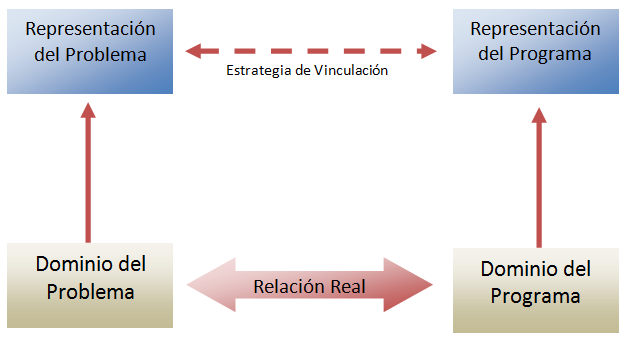
\includegraphics[scale= 0.50]{./dom.png}
\caption{Gráfico de Comprensión de Programas}
\end{figure} \label{captura1}

El inconveniente es que esta relación real es compleja de armar, por ende se puede bosquejar una aproximación mas accesible a través de los siguientes pasos: i) Elaborar una representación para el Dominio del Problema; ii)
Construir una representación del Dominio del Programa y iii) Elaborar un procedimiento de vinculación.
 
Para lograr con éxito los pasos antedichos se deben tener en cuenta conceptos muy importantes que son cimientos sobre los cuales esta sustentada la CP: los modelos cognitivos, la extracción de información, la interconexión de dominios y la visualización de software.

\section{Modelos Cognitivos}

Los \textit{Modelos Cognitivos} se refieren a las estrategias de estudio y las estructuras de información usadas por los programadores para comprender los programas. Estos modelos son importantes porque indican de que forma el programador comprende los sistemas y como incorpora nuevos conocimientos (aprende nuevos conceptos) \cite{MBPHRU10}.

Los modelos cognitivos abarcan 3 conceptos importantes: Conocimiento, un modelo mental y un proceso de asimilación \cite{MAS05}.

Existen 2 tipos de conocimientos uno es el conocimiento interno el cual se refiere al conocimiento que el programador ya posee antes de analizar el código del sistema de estudio. Por otro lado existe el conocimiento externo que representa un soporte de información externo que le brinda al programador nuevos conceptos. Los ejemplos mas comunes son la documentación del sistema, otros desarrolladores que conocen el dominio del problema, códigos de otros sistemas con similares características.

El concepto modelo mental hace referencia a representaciones mentales que el programador elabora en su mente al momento de estudiar el código del sistema. Estas representaciones mapean a distintas componentes del sistema. Algunos modelos construidos por los arquitectos del software como por ejemplo el \textit{Unified Modeling Language} UML, \textit{Entity Relationship} ER entre otros pueden verse como representaciones visuales de modelos mentales. 

Por último, el proceso de asimilación son las estrategias de aprendizaje que el programador usa para llevar adelante la comprensión de un programa. Los procesos de asimilación se pueden clasificar en tres grupos: Botton-up, Top-Down y distintas combinaciones de las anteriores(híbrida)\cite{MPOB03}.

El modelo de comprensión Botton-up indica que en primera instancia el código del sistema se lee por el desarrollador y luego el código se simplifica en un modelo mental, en pocas palabras se elabora una abstracción mental del código.

Por otro lado el modelo de comprensión top-down es una estrategia en donde primero el programador usa el conocimiento adquirido del dominio del problema para construir perspectivas del sistema en forma de modelo y luego estas perspectivas se vinculen con los distintos fragmentos del código.

Por ultimo el modelo híbrido que combina los dos conceptos mencionados top-down - bottom-up se adapta mucho mejor a los conocimientos que el programador posea durante el proceso de asimilación y con esto se logra mejores resultados.

Varios autores concluyen que estos conceptos conforman la base para encontrar la relación entre el dominio del problema y el dominio del programa \cite{TIE89,MPOB03}.

Para resumir sobre la temática de modelos cognitivos: el modelo mental es una representación mental que el programador tiene sobre el sistema. Si esta representación se la vincula con los conocimientos que el propio programador posee se logra un entendimiento completo del sistema como así también incrementa los conocimientos del programador. Con esto se deja en claro la importancia de modelos cognitivos en el proceso de entendimiento de los sistemas \cite{MBPHRU10}.

\section{Extracción de Información}

En la ingeniería del software existe una temática que se encarga de desarrollar/usar técnicas para la \textit{extracción de la información} en códigos de los sistemas, estas técnicas están catalogadas según el tipo de información que extraen.
Esta información puede ser: Estática o Dinámica, dependiendo de las necesidades del ingeniero de software o del equipo de trabajo. La principal diferencia que radica entre ambas técnicas es que las dinámicas requieren que el sistema se ejecute, mientras que las estáticas esto no es necesario.

La información estática esta contenida en el código fuente del sistema 
tipos, identificadores, procedimientos, y demás componentes visibles forman parte del código. Una estrategia para extraer la información estática consiste en utilizar técnicas tradicionales de compilación que extraigan los componentes del código deseados sin necesidad de ejecutar el programa.
%Para construir el analizador se suele utilizar una herramienta automatizada que lee una gramática y después genera el parser. En esta gramática asociada a un lenguaje particular se insertan acciones semánticas que formarán parte del parser generado.
Otra forma es usando grafo de llamadas a funciones en donde las aristas son funciones del programa de estudio y los arcos representan las llamadas entre dos funciones. A nivel conceptual es fácil de entender pero a veces la complejidad de los sistemas impiden una ágil realización sobre todo si los bloques de código tienen una complejidad temporal y espacial con cotas elevadas \cite{MBPHRU10}. Para la construcción de este grafo no se necesita ejecutar el programa.

Por otro lado la información dinámica se basa en elementos del programa presentes durante la ejecución del sistema. Para la extracción de este tipo de información se procede a bosquejar una técnica de instrumentación de código la cual consiste en insertar sentencias en el código sin modificar su semántica, así cuando el sistema se ejecute estas sentencias que contienen acciones se van a encargar de indicar que operaciones internas se llevaron a cabo para una determinada salida del programa.
La incorporación de estas sentencias debe realizarse con sumo cuidado y de forma estratégica para no alterar el flujo normal de ejecución.

Volviendo al objetivo principal que es aproximarse en la construcción de relación del dominio del problema con el dominio programa a través de representaciones esta requiere la extracción de información de ambos dominios.

La extracción de información del dominio del programa es una metodología sencilla de llevar a cabo por el hecho de que su extracción esta claramente marcada. El inconveniente radica en la extracción de la información perteneciente al dominio del problema, porque esta información es sensible a las características propias de la aplicación. Para encarar este inconveniente la ingeniería del software propone tomar las fuentes de información informal las cuales pueden estar presentes en el código por ejemplo: comentarios, literales string; o fuera del mismo: documentación, entrevistas con el cliente etc. Un vez que se extraen estos componentes se les puede aplicar alguna técnica de análisis de información informal para interpretar algunas las funcionalidades de los componentes del sistema.

Hasta aquí solo se ha mencionado estrategias de extracción información de los dominios del problema y del programa. Desafortunadamente el mapeo que relaciona la salida del sistema con los componentes que la integran queda a manos del programador y no abundan herramientas automatizadas que simplifiquen esta tarea.

\section{Estrategias de Interconexión de \\Dominios}

La \textit{Interconexión de Dominios} \cite{BRM10} tiene como principal objeto de estudio la transformación y vinculación de un dominio específico en otro dominio.
El punto importante es que cada componente de un dominio se vea reflejado en una o más componentes del otro y viceversa. 

Cuando se dice que relacionar el dominio del problema con el dominio del programa es importante ya que permite al desarrollador encontrar de forma mas ágil y rápida componentes en el software para una operación especifica. Esto facilidad impacta directamente en los tiempos dedicados a la evolución y al mantenimiento del software por el simple hecho de que se reduce la ardua tarea que tiene el programador de comprender el código.
Sin embargo solo se podrá destacar este impacto si el software de estudio es muy amplio y complejo.

%Los conceptos mencionados en los puntos anteriores como la visualización de software y la instrumentación de código forman la base para armar estrategias de interrelación de dominios.
A modo de ejemplo sobre interrelación de dominios, un caso es la transformación de un código fuente Dominio del Programa) en un Grafo de Llamadas a Funciones (Dominio de Grafos) como se mencionó en la sección anterior. Es importante aclarar que existe una amplia gama de transformaciones pero la más escasa y difícil de conseguir aquella que relaciona el Dominio del Problema con el Dominio del Programa.

Sin embargo actualmente existen técnicas recientemente elaboradas que conectan visualmente el dominio del problema y el dominio del programa usando la información estática y dinámica que se extrajo del sistema de estudio.

Una de las técnicas es \textit{Simultaneous Visualization Strategy} SVS, esta se encarga de mostrar los distintos componentes de un programa en plena ejecución, mediante distintas vistas, usando un inspector de sentencias, de esta manera se obtiene una visualización cuando el sistema se está ejecutando. Esta estrategia usa un esquema de instrumentación de código que se describió en párrafos precedentes, donde las acciones semánticas le van indicando a un visualizador la traza de invocaciones a funciones durante la ejecución del sistema \cite{BRM10,MPMR07}.

La otra estrategia se denomina \textit{Behavioral-Operational Relation Strategy} BORS, que a diferencia del SVS, espera a que termine la ejecución del sistema y luego la información recopilada por el instrumentador de código es procesada por BORS, entonces una abstracción gráfica del código ejecutado es devuelta por ejemplo como Árbol de Ejecución de Funciones. De esta forma se puede vincular mas claramente los conceptos del código capturados en tiempo de ejecución con la información asociada al dominio del problema \cite{BRM10,MPMR07}.

Existe también a nivel conceptual una técnica que combina ambas estrategias mencionadas llamada \textit{Simultaneous Visualization Strategy Improved} SVSI. Esta técnica disminuye los problemas que manifiestan tanto SVS como BORS y con ello se logra un mejor desempeño en cuanto a los resultados esperados \cite{BRM10,MPMR07}.

\section{Visualización de Software}

La \textit{Visualización del Software} es un pilar importante en la comprensión de programas, básicamente provee una o varias representaciones visuales (o vistas) de algún sistema particular. 

Existen distintos tipos de vistas, en si mismo, la primer vista de un sistema es el código en donde la información no esta tan clara para un desarrollador ajeno sobre todo si el software es grande y complicado. Es por eso que se necesita recurrir a otras vistas que representen una abstracción mas clara del sistema.
Las vistas poseen distintas características y para su construcción se requieren un conjunto de librerías gráficas. Dichas librerías son programas que simplifican la elaboración de las vistas y el diseñador de la visualización tiene la tarea de elegir que librería es la mas adecuada para la vista que desea construir. Las librerías gráficas mas conocidas son Jung, Prefuse, Graphviz y Cairo \cite{BRM10}. Las vistas cuando están bien construidas brindan una clara información del sistema y por ende facilita su comprensión. 

Los sistemas de visualización (SV) de software son herramientas útiles que se encargan de analizar los distintos módulos de un programa y generar vistas, dependiendo de la información que se desea visualizar existe una vista especifica \cite{MPMR07}. Cabe recordar que la información concebida en un sistema puede ser estática o dinámica.

Después de investigar distintos SV que actualmente existen: Myers, Price, Roman and Kenneth, Storey \cite{MBPHRU10}
en donde se concluye que la mayoría apuntan a capturar conceptos situados solo en el dominio del programa restando importancia al dominio del problema y a la relación entre ambos dominios. Debido a esta falencia Berón \cite{MBPHRU10} propone SV orientados a la CP ampliando aun mas los sistemas que hoy por hoy ya existen.

Para concluir se dice que la visualización de software orientada a la comprensión de programas tiene como principal desafío generar vistas que ayuden a relacionar el Dominio del Problema con el Dominio del Programa. 

\section{Comentarios}

Para resumir las ideas tratadas en este capítulo, comprender un programa se centra en la relación entre ambos dominios el del programa y del problema, como es demasiado complicado este vínculo, se llevan a cabo representaciones haciendo la \textit{extracción de información} correspondiente a cada dominio. Una vez construidas las representaciones de ambos dominios se procede a la elaboración de una estrategia de vinculación, el armado de esta estrategia se basa en los conceptos de \textit{interconexión de dominios}. Esta estrategia de vinculación ayuda al programador a entender con facilidad los programas ya que encuentra las partes del sistema que produjeron una determinada salida. La temática asociada a la \textit{Visualización del Software} indica que si se elaboran determinadas vistas se puede materializar gráficamente las representaciones de los dominios y la estrategia de vinculación (ver figura 2.1). Estas vistas ayudan a armar un puente cognitivo entre los aspectos del sistema y los conocimientos del programador, con esto se logra que el programador elabore una abstracción del sistema adecuada a su estructura mental.

Todos estos conceptos se deben tener en cuenta para uso/creación de Herramientas de Comprensión.
Las Herramientas de Comprensión son apropiadas para facilitar la comprensión de software ya que presenta diferentes perspectivas del sistema facilitando su análisis y su inspección.


%CAPITULO3=============================================================


\chapter{Análisis de Identificadores: Estado del Arte}

\lhead[]{CAPÍTULO 3. ANÁLISIS DE IDS: ESTADO DEL ARTE}

En el capítulo anterior se introdujo en el ámbito de comprensión de programas con las definiciones de los conceptos mas importantes. Este capítulo se centra en el estado del arte de técnicas que basan su análisis en los identificadores (ids) presentes en los códigos de los programas y también de algunas herramientas que implementan dichas técnicas.

\section{Introducción}

Los equipos de desarrollos de software frecuentemente enfocan todo su esfuerzo en el análisis, diseño, implementación y mantenimiento de los sistemas, restandole importancia a la documentación. Por lo tanto es común encontrar paquetes softwares carentes de documentación lo cual indica que la lectura de los códigos de los sistemas es la única manera de interpretarlos. Es necesaria la interpretación del sistema sobre todo en grandes equipos de desarrollo por el simple hecho de que un integrante del equipo puede tomar código ajeno para continuar con su desarrollo o realizar algún tipo de mantenimiento (Ver capítulo 2).

Como los códigos de los sistemas crecen a partir de los nuevos requerimientos y el frecuente mantenimiento, esto implica que cada vez mas los sistemas se hacen mas complejos y difíciles de entenderlos. He aquí la importancia del uso de las herramientas de comprensión, con ellas se puede lograr un entendimiento ágil y facilitar las arduas tareas de interpretación de códigos.

Como se mencionó en el capítulo anterior la CP desarrolla métodos, técnicas y herramientas que facilitan al programador entender los programas.

La extracción de información estática es un aspecto importante de la CP (Capítulo 2) en donde se pueden aplicar técnicas de compilación conocidas para extraer información oculta detrás de los componentes visibles en los códigos de los programas sin necesidad de ejecutarlos. Uno de los componentes mas importantes presentes en los códigos de los sistemas que contienen información oculta son los identificadores (ids).

El la siguiente tabla se muestra un análisis léxico que se realizó sobre 2.7 millones de lineas de códigos escritos en lenguaje JAVA.\\

\begin{center}
   \begin{tabular}{| l | c | c | c | c | }
     \hline
     \textsf{Tipo} & \textsf{Cantidad} & \textsf{\%} & \textsf{Caracteres} & \textsf{\%} \\ \hline
     Palabras claves & 1321005 & 11.2 & 6367677 & 12.7 \\ \hline
     Delimitadores & 5477822 & 46.6 & 5477822 & 11.0 \\ \hline
     Operadores & 701607 & 6.0 & 889370 & 1.8 \\ \hline
     Literales & 378057 & 3.2 & 1520366 & 3.0 \\ \hline          
     \textbf{Identificadores} & 3886684 & 33.0 & \textbf{35723272} & \textbf{71.5} \\ \hline
     \textbf{Total} & \textbf{11765175} & \textbf{100.0} & \textbf{49978507} & \textbf{100.0} \\ \hline          
   \end{tabular}
\end{center}


Se ve claramente que mas de las dos terceras partes (71.5\%) de los caracteres en el código fuente forman parte de un id\cite{DFPM05,DMDJ13}. 

Por ende en el ámbito de CP los ids son una fuente importante de información que el lector del código o encargado de mantenimiento debe tener en cuenta. Utilizar una herramienta que analice los ids dando a conocer su significado ayuda a revelar esta información, mejora la comprensión, aumenta la productividad y agiliza el mantenimiento de los sistemas.

Para finalizar construir herramientas de CP que se encargan de analizar ids en los códigos fuentes de los programas es una tarea importante de llevar a cabo.

\section{Conceptos claves}

%whats the name - Lawrie
Existen dos fuentes importantes de información que se encuentran dentro de los códigos de los programas una son los comentarios y la otra son los ids. Cuando en el código no abundan los comentarios la única fuente son los ids.

\begin{verse}
\textbf{Identificador (id)}: básicamente se define como una secuencia de letras, dígitos o caracteres especiales de cualquier longitud que sirve para identificar las entidades del programa (clases, funciones, variables, tipos estructurados, etc.). 
Cada lenguaje tiene sus propias reglas que definen como pueden estar construidos sus nombres. Por lo general lenguajes como C y JAVA no esta permitido declarar ids que coincidan con palabras reservadas o que contengan símbolos especiales (\$,\&,\#, etc).
\end{verse}


Un id en un programa esta asociado a un concepto del programa. 

\begin{center}
\textsf{Identificador $\Leftrightarrow$ Concepto}
\end{center}

Dicho de otra manera un id es un representante de un concepto ubicado en el dominio del problema\cite{DFPM05,DMDJ13}.%mas biblografia

%whats the name - Lawrie
Para mejorar la CP se requiere que los nombres de los ids comuniquen de manera clara los conceptos que representan\cite{DCHD06}. Sin embargo esto no sucede frecuentemente. En la siguiente sección se menciona como el nombramiento de los ids impacta enormemente en la lectura comprensiva del código fuente. 


\pagebreak
\section{Nombramiento de Identificadores}

%Deißenbock and Pizka DFPM05
%Intro
Durante los desarrollos de los sistemas, las reglas de nombramiento de ids se enfocan más en el formato del código y en la documentación en lugar de enfocarse en el concepto que el id representa. Luego durante la etapa de mantenimiento del software la forma en la que los ids están nombrados no es muy tenida en cuenta para comprender el sistema.

Estudios realizados sobre 100 programadores\cite{DCHD06} sobre comprensión de ids indican que existen tres tipos principales de nombramiento en los ids (entre paréntesis se da el ejemplo asociado al concepto \textsf{File System Input}): 

\begin{itemize}
\itemsep0em%reduce espacio
\item Palabras completas (\textsf{fileSystemInput}).
\item Abreviaciones (\textsf{flSysIpt}).
\item Una sola letra (\textsf{fsi}). 
\end{itemize}

De mas esta decir que los nombres de los ids pueden estar compuestos por mas de una palabra.

El estudio arrojó que las palabras completas son las mas comprendidas, sin embargo las estadísticas marcan en algunos casos que las abreviaciones que se ubican en segundo lugar no demuestran una diferencia notoria con respecto a las palabras completas\cite{DCHD06}. 


Los autores Feild, Binkley, Lawrie \cite{FBL06,HDD06,DMDJ13} distinguen 2 formas de nombramiento en los ids conocidas como \textit{hardwords} y \textit{softwords}. Los hardwords destacan la separación de cada palabra que compone el identificador a través de una marca específica; algunos ejemplos son: \textsf{fileSystem} marca bien la separación de cada palabra con el uso de mayúscula entre las minúsculas\footnote[1]{Algunos autores lo llaman camel-case a este nombramiento} o \textsf{fileSYSTEM} así también como utilizar un símbolo especial como es el caso del guion bajo \textsf{file\_system}. En cambio los softwords no poseen ningún tipo de separador o marca que de indicios de las palabras que lo componen; por ejemplo: \textsf{textinput} esta compuesta por \textsf{text} y por \textsf{input} sin tener una marca que destaque la separación.

Si bien en el párrafo anterior se dio una taxonomía de como se clasifican los ids, en los ejemplos no se refleja como normalmente se nombra un id.
Generalmente los programadores para reducir el esfuerzo de tipeo escriben los ids en forma abreviada compuestos por mas de una palabra, esto se lo conoce con el nombre de acrónimos. Para dar un ejemplo sobre esto: el id \textsf{fileSystem} los programadores lo suelen nombran como \textsf{flSys}, \textsf{fiStm}, \textsf{fl\_sys} u otras tantas posibles representaciones abreviadas.

%Caprile and Tonella state that “identifier names are one of the most important sources of information about program entities”\cite{BCPT00}

%Caprile and Tonella - Software entities are born and live with their names. \cite{BCPT99}

%================================

En la actualidad existen innumerables convenciones en cuanto al nombramiento de los ids, alguna de ellas son:

\begin{itemize}
\itemsep0em%reduce espacio
\item En el caso de JAVA\texttrademark los nombres de los paquetes deben ser con minúscula (main.system) y las clases con mayúscula en la primer letra de cada palabra que compone el nombre (MainClass).

\item En el caso de C\#\texttrademark las clases se nombran igual que JAVA\texttrademark pero los paquetes en cada nivel de nombre debe comenzar con mayúscula y resto minúscula (Main.System).
\end{itemize}

Esto indica que se concentra mas en los aspectos sintácticos del id y no tanto en los aspectos semánticos en lo que respecta al nombramiento. 

%Las investigaciones realizadas por Deissenboeck y Pizka \cite{DFPM05} a este problema parte de que cada nombre de id esta asociado a un concepto del dominio del problema y viceversa. 
%Mas formalmente se puede ver como una función biyectiva:

%\begin{center}
%\textsf{Nombre $\Leftrightarrow$ Concepto}
%\end{center} 

%En este contexto se dice que se logra un nombramiento conciso y consistente de ids. 

%Problema: de porque no existe un correcto nombramiento
Una evidencia fehaciente de la importancia en el buen nombramiento son las técnicas que se aplican para protección de código, algunas de ellas se encargan de reemplazar los nombres originales de los ids por secuencias de caracteres aleatorios 
para reducir la comprensión, esta se conocen con el nombre de ofuscación de código. La ofuscación es común en los sistemas de índole comercial, en la figura \ref{captura2} se puede observar un ejemplo tomado de un caso real en donde la función \textsf{mr\_mr\_1} no parece complicada pero se desconoce la finalidad de su ejecución\cite{DFPM05}.

\begin{figure}[t] %[h] para here [b] para bottom [t] para top
\centering
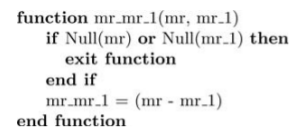
\includegraphics[scale= 0.70]{./idd_1.png}
\caption{Trozo de Código de un Sistema Comercial}
\label{captura2}
\end{figure}



Existen tres razones destacadas que conllevan al mal nombramiento:

\begin{enumerate}
\itemsep0em%reduce espacio
\item Los ids son escogidos por los desarrolladores y eluden el análisis automático.

\item Los desarrolladores tienen poco conocimiento de los nombres usados en los ids ubicados en otros sectores del código fuente.

\item Durante la evolución del sistema los nombres de los ids se mantienen y no adaptan sus nombres a las nuevas funcionalidades que pueden tener.
\end{enumerate}

En este sentido el mal nombramiento de los ids se combate con la programación “menos egoísta” que consiste en hacer programas mas claros y entendibles para el futuro lector que no esta familiarizado con el mismo.

%Otro concepto importante es la consistencia de nombres en los ids dentro de un sistema:

%\noindent remueve la sangria!
\begin{framed}
\noindent \textbf{Conciso:} El nombre de un id es conciso si la semántica del nombre coincide exactamente con la semántica del concepto que el id representa.

\noindent \textbf{Consistente:} Para cada id debe tener asociado si y solo si un único concepto.
\end{framed}

Por lo tanto si los ids están bien nombrados y la consistencia esta presente se pueden descubrir los conceptos que representan en el dominio del problema mas fácilmente y de esta manera agiliza la comprensión del código, aumenta la productividad, mejora la calidad durante la etapa de mantenimiento \cite{DFPM05}.%agregar mas bibliografia



En la practica es muy difícil mantener una consistencia global de nombres en los ids durante las etapas de desarrollo y mantenimiento del software, sobre todo si este es muy grande. Cada vez que un concepto se modifica el nombre del id asociado debe cambiar y adaptarse a la modificación pero esto no ocurre frecuentemente en la practica.

%sinonimos y homonimos
Otra amenaza que atenta contra las “buenas constumbres” de nombramiento en los ids son conocidas en el lenguaje natural con el nombre de sinónimos y homónimos. Cabe recordar que para mantener una consistencia de nombres en los ids, para cada id debe existir si y solo si un concepto. Los homónimos son palabras que pueden tener mas de un significado por ende el concepto al que esta asociado no esta muy claro (Ej: un id con el nombre `file' generalmente se asocia al concepto de archivo pero puede que se refiera a una estructura o a una fila de una tabla). Por otro lado los sinónimos indican que para un mismo concepto pueden tener asociados diferentes nombres (Ej: un id con el nombre `accountNumber' y otro `account' hacen referencia al mismo concepto `numero de cuenta bancaria'). Esta demostrado que los códigos con mucha presencia de estos casos mencionados hacen que se dificulte identificar con claridad los conceptos en el código y por ende aumenta los esfuerzos de comprensión del programa.

Intuitivamente se concluye 	que mientras mejor nombrado estén los ids con respecto al concepto que representa, mayor es el impacto que tendrá en la interpretación del sistema\cite{DFPM05}.

%solucion propuesta
Los autores Deissenboeck y Pizka\cite{DFPM05} proponen utilizar una herramienta que solucione los problemas de mal nombramiento planteados anteriormente, dado la dificultad que conlleva a la construcción de una herramienta totalmente automática que se encargue de nombrar correctamente los ids se elaboró una herramienta semi-automática que necesita la intervención del programador. Esta herramienta construye y mantiene un diccionario de ids a medida que el sistema se va desarrollando. Cabe destacar el concepto de diccionario en el contexto de ingeniería de software.

\begin{verse}
\textbf{Diccionarios de Datos:} Este concepto conocido también como `glosario de proyecto' se recomienda en los textos orientados a la administración de proyectos de software. Con los diccionarios se describe en forma clara todos los términos utilizados en los grandes sistemas de software y con esto se brinda una referencia completa a todos los participantes de un proyecto durante todo el ciclo de vida del producto.
\end{verse}

A continuación se describe una herramienta que ayuda al buen nombramiento de ids y mantiene la consistencia de nombres.

\begin{figure}[h] %[h] para here [b] para bottom [t] para top
\centering
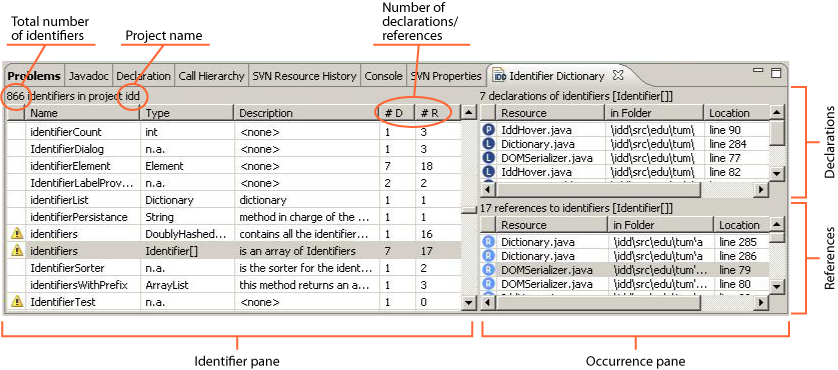
\includegraphics[scale= 0.50]{./idd_2.png}
\caption{Visualización de Identifier Dictionary}
\label{captura3}
\end{figure}
\pagebreak
\subsection{Identifier Dictionary}

La herramienta conocida con el nombre de identifier dictionary (IDD)\footnote[1]{http://www4.informatik.tu-muenchen.de/\~{}ccsm/idd/index.html} básicamente actúa como un diccionario de datos que ayuda al desarrollador a mantener la consistencia de nombres en los ids de un proyecto JAVA. Es una base de datos que almacena información de los ids tales como el nombre, el tipo del objeto que identifica y una descripción comprensiva.

Ayuda a reducir la creación de nombres sinónimos y ayuda a escoger un nombre adecuado para los ids siguiendo el patrón de nombres existentes. Aumenta la velocidad de comprensión del código en base a las descripciones de cada id. El equipo encargado de tareas de mantenimiento localiza un componente del domino del problema y luego su correspondiente id de manera ágil. Otro aporte que hace la herramienta es asegurar la calidad de los nombres de los ids con un esfuerzo moderado usando como ayuda la descripción comprensiva.

Se implementó como extensión de la IDE Eclipse 3.1\footnote[2]{http://www.eclipse.org/jdt}. Se visualiza en el panel de las vistas de la IDE y consiste de tres secciones (Figura \ref{captura3}):

\begin{figure}[t] %[h] para here [b] para bottom [t] para top
\centering
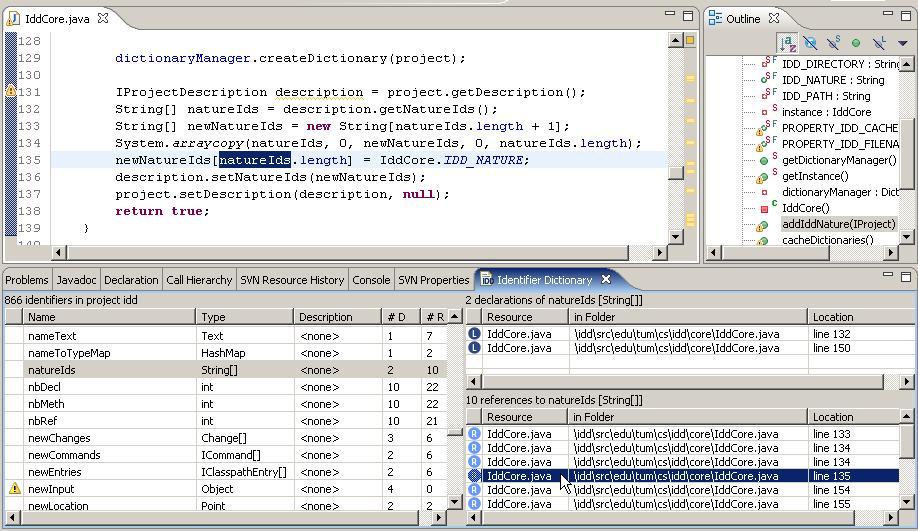
\includegraphics[scale= 0.46]{./idd_3.png}
\caption{Visualización de Identifier Dictionary}
\label{captura4}
\end{figure} 

\begin{itemize}
\itemsep0em%reduce espacio
\item Tabla con información de los ids en el proyecto: nombre, tipo, descripción, cantidad de declaraciones y cantidad de referencias. (Indentifier pane).
\item Lista de Ids declarados en el proyecto (Ocurrence pane).
\item Lista de referencias de los ids en el proyecto (Ocurrence pane).
\end{itemize}

Mientras se realiza el desarrollo del código la herramienta ayuda al programador a llevar un buen nombramiento en los ids a través de las siguientes características:

\textbf{Navegación en el código fuente:} Si se selecciona un id en la tabla de ids (izquierda), la parte derecha mostrará las declaraciones y las referencias de ese id mostrando en las columnas de la derecha la ubicación exacta en donde se encuentra cada declaración y referencia.(Figura \ref{captura4}).


%\begin{figure}[h] %[h] para here [b] para bottom [t] para top
%\centering
%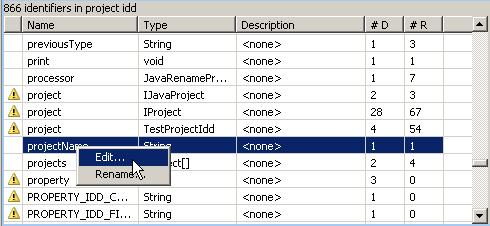
\includegraphics[scale= 0.55]{./idd_4.png}
%\caption{Visualización de Identifier Dictionary}
%\label{captura5}
%\end{figure}
%
%\textbf{Guardar descripción:} Botón derecho en el panel de ids y luego en edit. Permite agregar una descripción comprensiva (Figura \ref{captura5}).

%\begin{figure}[h] %[h] para here [b] para bottom [t] para top
%\centering
%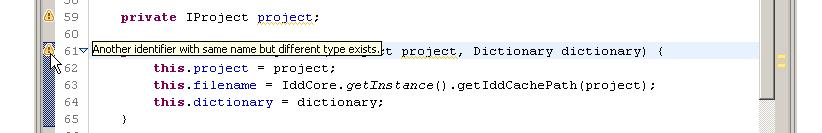
\includegraphics[scale= 0.55]{./idd_5.png}
%\caption{Visualización de Identifier Dictionary}
%\label{captura6}
%\end{figure}
\begin{figure}[t] %[h] para here [b] para bottom [t] para top
\centering
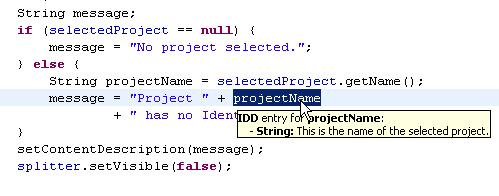
\includegraphics[scale= 0.80]{./idd_7.png}
\caption{Visualización de Identifier Dictionary}
\label{captura8}
\end{figure}

\textbf{Advertencias (warnings):} Mientras se realiza la colecta de ids los iconos de advertencia indican potenciales problemas en el nombramiento.  Los dos tipos de mensajes que se muestran son: dos ids con el mismo nombre pero distinto tipos y el id es declarado pero no referenciado.


%\begin{figure}[h] %[h] para here [b] para bottom [t] para top
%\centering
%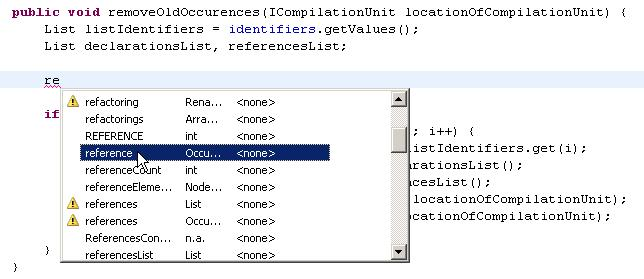
\includegraphics[scale= 0.55]{./idd_6.png}
%\caption{Visualización de Identifier Dictionary}
%\label{captura7}
%\end{figure}

\textbf{Mensajes pop-up:} Se puede visualizar la información posicionando el cursor sobre el id en el código fuente mientra se esta programando (Figura \ref{captura8}).

\textbf{Auto-completar nombres:} Las IDE actuales proveen la función de auto-completar. Sin embargo esta funcionalidad falla cuando los nombres de los ids no están declarados dentro del alcance actual de edición. Idd no tiene en cuenta el alcance desde el lugar que se esta editando, ademas de considerar el nombre del id también considera el tipo al momento de auto-completar.

%\begin{figure}[h] %[h] para here [b] para bottom [t] para top
%\centering
%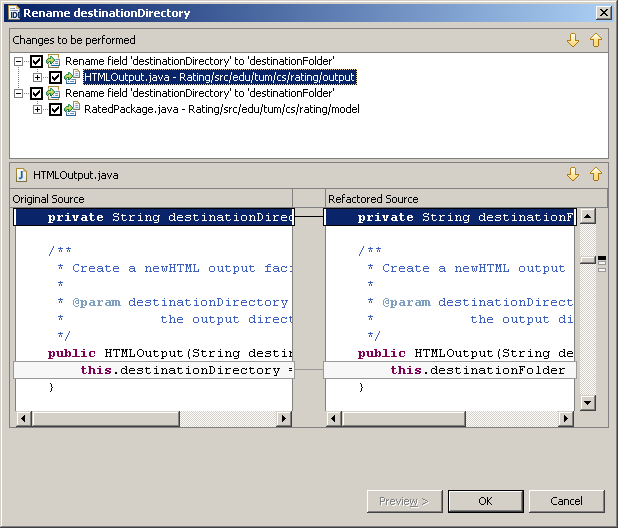
\includegraphics[scale= 0.55]{./idd_8.png}
%\caption{Visualización de Identifier Dictionary}
%\label{captura9}
%\end{figure}

\textbf{Renombre global de ids:} Esta función permite renombrar cualquier id generando una vista previa y validando el nombre de los ids a medida que sistema va evolucionando. De esta forma se preserva la consistencia de nombres.

La herramienta idd trabaja internamente con un colector de ids que esta acoplado al proceso de compilación del proyecto(build proyect) de Eclipse. Los ids se van recaudando a medida que el programa se va compilando. Los nombres, el tipo, la descripción se van guardando en un archivo XML. También se puede exportar en un archivo en formato HTML el cual permite una lectura más clara de los ids con toda información asociada\cite{DFPM05}.


%%=========Lawrie

Para concluir la buena calidad en el nombramiento de los ids descripta anteriormente no solo mejora el entendimiento del código sino que también abre la posibilidad de construir herramientas que ejecuten técnicas de regresión para traducir los nombres de los ids a palabras conocidas. En la sección siguiente se dan a conocer casos que utilizan estas técnicas de regresión.

%%=====================================
\pagebreak
\section{Análisis de Identificadores}

Los lectores de códigos de programas tienen inconvenientes para entender el propósito de los ids y deben invertir tiempo en analizar el significado de su presencia. Estrategias automáticas dedicadas a facilitar este análisis son bienvenidas en el contexto de la CP.

La literatura correspondiente a estrategias de análisis de ids indican que los ids ocultan información relevante del domino del problema detrás de sus abreviaturas\cite{EHPV09,LFBEX07}. 

Una manera de desplegar esta información oculta es intentar convertir estas abreviaturas en palabras completas del lenguaje natural. Por ende el foco del análisis de los ids se basa en la traducción de palabras abreviadas a palabras completas.

El proceso que se lleva a cabo para realizar la traducción mencionada:

\begin{enumerate}
\itemsep0em%reduce espacio
\item \textbf{División:} Separar el id en las palabras que lo componen usando algún separador especial. (Ejemplo: \textsf{flSys} $\Rightarrow$ \textsf{fl-sys}).

\item \textbf{Expansión:} Expandir las abreviaciones que resultaron como producto del paso anterior. (Ejemplo: \textsf{fl-sys} $\Rightarrow$ \textsf{file system}).
\end{enumerate}

Tanto los nombres de los ids como las abreviaturas utilizadas en ellos dependen mucho de la idiosincrasia del programador y esto representa un verdadero desafío para las herramientas de análisis de ids.

%Como bien se describió en la sección es importante 






%tonella-caprile
\pagebreak 
\subsection{Identifier Restructuring Tool}

\begin{figure}[h] %[h] para here [b] para bottom [t] para top
\centering
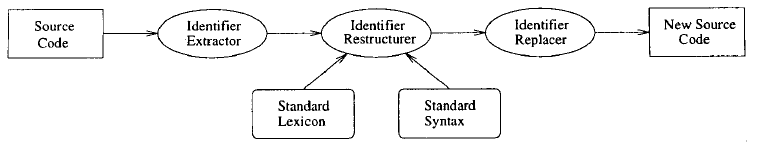
\includegraphics[scale= 0.80]{./ire_1.png}
\caption{Etapas de Restructuring tool}
\label{ire1}
\end{figure}

La herramienta restructuring tool\cite{BCPT00} se encarga de recibir como entrada un código fuente escrito en lenguaje C y luego a través de un proceso de transformación cada nombramiento de los id se expande a palabras completas, retornando de esta manera el mismo código pero con los ids expandidos.
El código fuente se convierte de esta manera en un código mas entendible y mejora la comprensión. El proceso consta de tres etapas (Figura \ref{ire1}): 

\begin{enumerate}
\itemsep0em%reduce espacio
\item \textbf{Identifier Extractor:} Recupera una lista con los nombres de los ids presentes en el código. Este modulo se programó con un parser modificado de C que reconoce los ids y los extrae.
\item \textbf{Identifier Restructurer:} Genera una asociación entre el nombramiento actual del id y un nombramiento estándar expandido y más claro. El primer paso consiste en segmentar el id en las palabras que lo constituyen, después cada palabra se expande usando un diccionario de palabras estándar (estándar léxico) y finalmente la secuencia de palabras en los ids deben coincidir con reglas predefinidas por una gramática para determinar que acción cumple cada id en el código (estándar sintáctico).
\item \textbf{Identifier Replacer:} Transforma el código original en el nuevo código usando las asociaciones que se construyeron en la etapa anterior. Se emplea un scanner léxico para evitar reemplazar posibles nombres de ids contenidos en literales strings y en comentarios.
\end{enumerate}

Los pasos 1 y 3 están totalmente automatizados. Sin embargo no sucede lo mismo con el paso 2 porque se necesita la intervención del programador para lograr una expansión adecuada de nombres.

\begin{figure}[h] %[h] para here [b] para bottom [t] para top
\centering
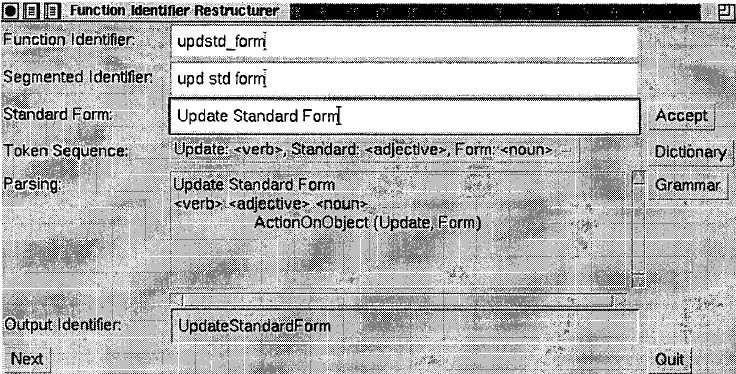
\includegraphics[scale= 0.60]{./ire_2.png}
\caption{Etapas en la transformación del id.}
\label{ire2}
\end{figure}

\begin{figure}[t] %[h] para here [b] para bottom [t] para top
\centering
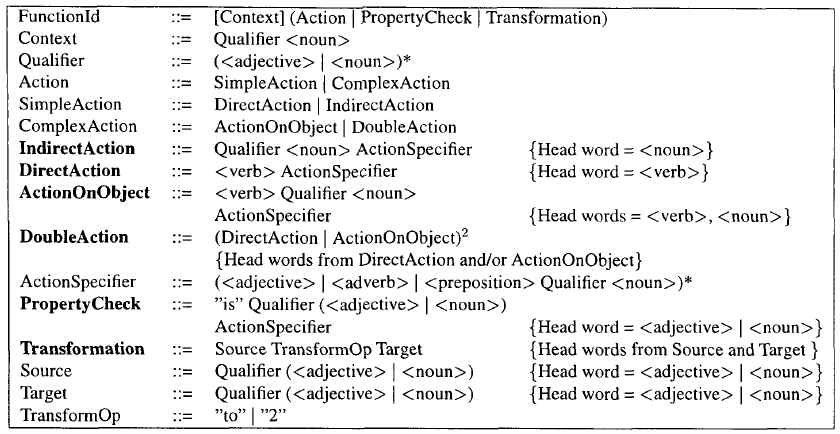
\includegraphics[scale= 0.70]{./ire_3.png}
\caption{Gramática que determina la función de los ids.}
\label{ire3}
\end{figure}

A continuación se detalla el paso 2 que es el mas importante de esta herramienta (Figura \ref{ire2}).

\begin{description}
\itemsep0em%reduce espacio
\item[Segmentation:] El id es separado en las palabras que lo componen. De manera automática se utilizan estrategias de separación (basada en guion bajo o camel-case) así como un diccionario para reconocer cada palabra. El algoritmo toma un string \textit{s} como entrada, utiliza una estrategia greedy verificando a partir de la primer letra de \textit{s} un sub-string que pertenezca en el diccionario, luego el sub-string se descarta y continua el análisis con el resto hasta que no haya mas sub-strings que separar\cite{BCPT99}.

\item[Standard Lexicon:] Una vez lograda la separación de las palabras estas son mapeadas a una forma estándar con la ayuda de un diccionario léxico\cite{BCPT99}. Este diccionario puede ser definido por el usuario al igual que el procedimiento para actualizarlo. En caso de que no exista una asociación, opcionalmente además se puede construir un diccionario de sinónimos con términos extraídos del código fuente que se consideran estándares. Para comenzar el análisis los autores\cite{BCPT00} de la herramienta construyeron los diccionarios de manera genérica tomando como muestra 10 programas. Sin embargo con el tiempo los diccionarios deben crecer con la inclusión de nuevos términos.

\item[Tokenization:] Una vez obtenidas las palabras a una forma estándar en el paso anterior, se procede a asignar cada palabra a un \textit{tipo léxico} (verbo, sustantivo, adjetivo). Por ejemplo la palabra Update $\rightarrow$ $<$Update,verb$>$ y Standard $\rightarrow$ $<$Standard,adjective$>$. Esta tuplas se denominan tokens y se utiliza un `diccionario de tipos' para generarlos de manera automática, este diccionario al igual que los otros se arma previamente a gusto del programador\cite{BCPT99}. Sin embargo existen casos que se necesita la intervención humana para determinar el tipo correcto, por ejemplo: free en ingles es un verbo, adjetivo y a la vez un adverbio en este caso la herramienta va a elegir lo que el diccionario le indique (si free esta presente).

\item[Parsing:] Finalmente la secuencia de tokens obtenidos en la etapa anterior se parsea usando una gramática predefinida para determinar cual es el rol/acción del id en código fuente de esta manera se determina la acción semántica del id. Esta gramática puede ser construida por el usuario, en la figura \ref{ire3} se muestra la desarrollada por los autores. Es una gramática regular donde los símbolos terminales están indicados con $<>$, las producciones con negrita indican distintos tipos de ids donde el verbo expresa la acción y el sustantivo representa al objeto de la acción, por ejemplo \textbf{ActionOnObject} $\Rightarrow$ go,home $\equiv$ $<$verb$>$,$<$noun$>$.

En caso de que el parseo falle el proceso se reinicia desde el comienzo partiendo nuevamente de la etapa de segmentación\cite{BCPT00} (figura \ref{ire2}).
\end{description}

\begin{figure}[t] %[h] para here [b] para bottom [t] para top
\centering
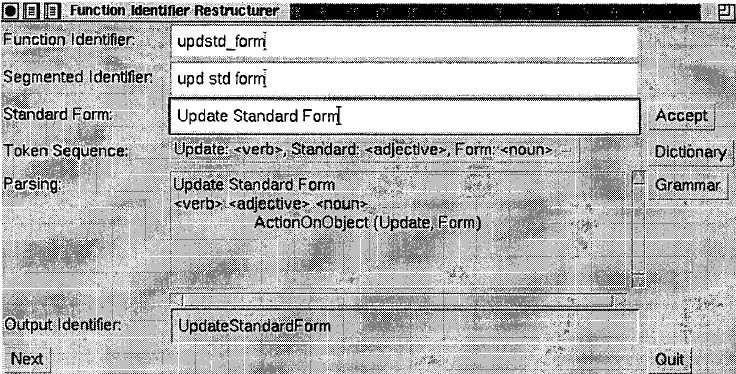
\includegraphics[scale= 0.80]{./ire_4.png}
\caption{Visualización de Restructuring Tool.}
\label{ire4}
\end{figure}

La interfaz de usuario de \textbf{Identifier Restructurer} se visualiza en la figura \ref{ire4}, el id de entrada se muestra en el primer cuadro de texto \textsf{updstd\_form}. Se usa heurísticas sencillas(guión bajo, camel-case) para separar las palabras del id, en este caso \textsf{updstd} y \textsf{form}. Como esta segmentación esta incompleta el usuario puede separar manualmente en el segundo cuadro de texto la palabra \textsf{upd} y \textsf{std}. En el tercer cuadro de texto se propone la forma estándar de cada palabra. Cuando una palabra no se puede expandir la herramienta muestra un signo de pregunta en su lugar (?). En este caso \textsf{upd} $\rightarrow$ \textsf{Update}, \textsf{std} $\rightarrow$ (?), \textsf{form}$\rightarrow$ \textsf{Form}, como \textsf{std} no esta presente en el diccionario se necesita la intervención del desarrollador para que se complete correctamente a  \textsf{Standard}. Luego las palabras expandidas son asociadas a la función gramatical. En esta etapa puede existir para una secuencia de palabras mas de una función gramatical(la gramática es ambigua y puede generar mas de una secuencia de tokens). En caso de suceder esto el usuario puede elegir cual es la secuencia mas adecuada, en el ejemplo no ocurre esto y la única posibilidad es mostrada en el cuarto cuadro de dialogo(figura \ref{ire4}). Finalmente el resultado se muestra en en cuadro de texto de mas abajo, en el cuadro de Parsing se puede apreciar la acción que aplica el id, en este caso \textbf{ActionOnObject(Update,Form)} `actualizar formulario'.

Cuando se arma la asociación de los nombres ids con los nuevos nombres generados la misma debería cumplir con la propiedad de inyectividad, de esta forma se evita que haya conflictos de nombres entre los distintos ids del programa. Al final de esta etapa la herramienta ayuda al programador a conseguir este objetivo resaltando los posibles conflictos en los nombres.



%Con este estudio se puede observar que los ids son una fuente importante de información, por eso elaborar técnicas que analicen ids es un aporte destacado para la CP.

%\section{Técnicas de División de Identificadores}
%\section{Técnicas de Expansión de Identificadores}

%En el área de Ingeniería del Software, existen herramientas automatizadas que permiten hacer análisis de los identificadores utilizados en los códigos de programación. Estas herramientas extraen parcialmente conceptos representados en los identificadores del código fuente para intentar interpretar lo que el programador quiso desarrollar.

%Estas técnicas exhiben información estática oculta detrás de los ids, esta información es importante porque da indicios de lo que un sistema realiza en su ejecución por ende es un aporte en el ámbito de Comprensión de Programas. --colocar abajo

%========================================================================
\bibliographystyle{plain}%{alpha}
\bibliography{biblo.bib}

\end{document}
